\documentclass{standalone}
\usepackage{tikz}
\usepackage{amssymb}
\usepackage{bm}
\usepackage{graphicx}
\usepackage{color}
\usepackage{tikz}
\usetikzlibrary{arrows}
\begin{document}
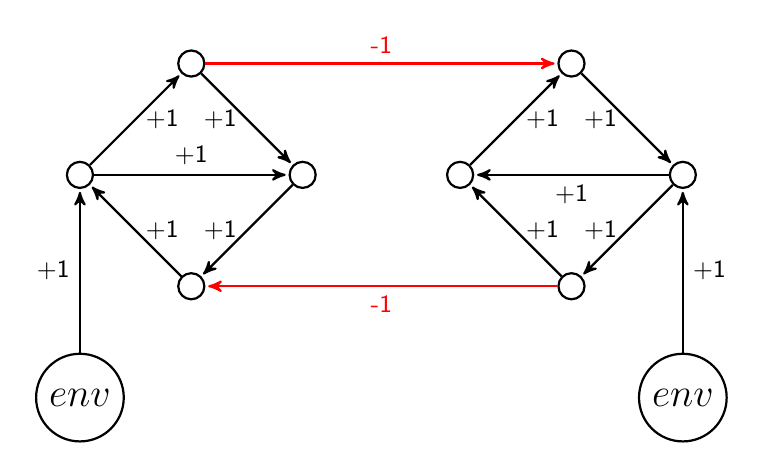
\begin{tikzpicture}[->,>=stealth',shorten >=1pt,auto,node distance=2.cm,
                    thick,main node/.style={circle,draw,font=\sffamily\Large\bfseries}]

  \node[main node] (1) {};
  \node[main node] (2) [below left of=1] {};
  \node[main node] (3) [below right of=2] {};
  \node[main node] (4) [below right of=1] {};
  \node[main node] (5) [right of=4] {}; 
  \node[main node] (6) [below right of=5] {};
  \node[main node] (7) [above right of=6] {};
  \node[main node] (8) [above left of=7] {};
  \node[main node] (9) [below left of=3] {$env$};
  \node[main node] (10) [below right of=6] {$env$};

\path[every node/.style={font=\sffamily\small}]
    (1) edge node [left] {+1} (4)
         edge [red] node {-1} (8)
    (2) edge node [right] {+1} (1)
         edge node {+1} (4)   
    (3) edge node [right] {+1} (2)
    (4) edge node [left] {+1} (3)
    (8) edge node [left] {+1} (7)
    (5) edge node [right] {+1} (8) 
    (6) edge node [right] {+1} (5)
        edge [red] node {-1} (3)
    (7) edge node [left] {+1} (6)
            edge node {+1} (5)  
    (9) edge node [left] {+1} (2)
    (10) edge  node [right] {+1} (7);




\end{tikzpicture}
\end{document}
